%% Простая презентация с примером включения программного кода и
%% пошаговых спецэффектов
\documentclass{beamer}
\usepackage{fontspec}
\usepackage{xunicode}
\usepackage{xltxtra}
\usepackage{xecyr}
\usepackage{hyperref}
\setmainfont[Mapping=tex-text]{DejaVu Serif}
\setsansfont[Mapping=tex-text]{DejaVu Sans}
\setmonofont[Mapping=tex-text]{DejaVu Sans Mono}
\usepackage{polyglossia}
\setdefaultlanguage{russian}
\usepackage{graphicx}
\usepackage{listings}
\lstdefinestyle{mycode}{
  belowcaptionskip=1\baselineskip,
  breaklines=true,
  xleftmargin=\parindent,
  showstringspaces=false,
  basicstyle=\footnotesize\ttfamily,
  keywordstyle=\bfseries,
  commentstyle=\itshape\color{gray!40!black},
  stringstyle=\color{red},
  numbers=left,
  numbersep=5pt,
  numberstyle=\tiny\color{gray},
}
\lstset{escapechar=@,style=mycode}


\addtobeamertemplate{navigation symbols}{}{%
    \usebeamerfont{footline}%
    \usebeamercolor[fg]{footline}%
    \hspace{1em}%
    \insertframenumber/\inserttotalframenumber
}



\usepackage{graphicx}       % работа с картинками
\usepackage[export]{adjustbox}  % еще про место картинки (width,right/left])
\usepackage{multicol,caption,float, subfig} % картинки

\usepackage{multirow} % для няшных табличек       

\captionsetup[subfigure]{labelformat=empty}

\begin{document}
    \title{Рекомендательная система для Stepic.org}
    \author{Лена Волжина\\{\footnotesize\textcolor{gray}{кураторы: Андрей Баландин, Николай Вяххи}}}
    %\institute{СПбГУ}
    \date{весна 2016}     % можно поставить какую-нибудь дату
\frame{\titlepage}



\begin{frame}\frametitle{Введение}  % все знают, что такое stepic
    \begin{figure}[H]
    \center{
\includegraphics[width=\linewidth]{images/stepic_youtube.PNG}}
    \end{figure}
\end{frame}




\begin{frame}\frametitle{Рекомендательная система: что уже было сделано}
% хотим рекомендовать пользователю интересные ему уроки
% мы знаем о пользователе ВСЁ
    Информация о пользователе:
    \begin{itemize}
        \item просмотренные уроки   % какие уроки он смотрел
        \item теги этих уроков      % какие теги ему интересны
        \item незаконченные уроки  % какие уроки он не досмотрел
        \item откуда он пришел, какой у него уровень, как давно он на платформе, ...
    \end{itemize}
    \bigskip
    Что еще знаем:
    \begin{itemize}
        \item пути по урокам    % чаще всего совпадающие с курсами
        \item process map по урокам     % куда перейти с текущего урока
        \item process map по тегам      % схожесть между тегами
        \item схожесть между пользователями (коллаборативная фильтрация)
    \end{itemize}
\end{frame}


\begin{frame}\frametitle{Рекомендательная система: хендлеры}
% придумали несколько сценариев (user case), на каждый свой обработчик (handler)
% каждый хендлер продуцирует список уроков с весами от 0 до 1
    \begin{figure}[H]
    \center{\includegraphics[width=\linewidth]{images/handlers_scheme.png}}
    \end{figure}
% какие-то хендлеры более персонализированны, какие-то менее
\end{frame}



\begin{frame}\frametitle{Что было сделано в рамках данной практики}

    \begin{itemize}
        \item Контекстные рекомендации (дополнительные хендлеры)
        \bigskip
        \item Адаптивные рекомендации
        \bigskip
        \item Замеры эффективности
    \end{itemize}

\end{frame}



\begin{frame}\frametitle{Адаптивные рекомендации: \\MathsGarden}

    \bigskip
    MathsGarden.com\cite{mathsgarden}
    
    \begin{itemize}
        \item Elo chess rating
        \item Item Response theory
        \item High speed, high stakes
    \end{itemize}
    
    \begin{figure}[t]
      \centering
      \subfloat[начальный экран]{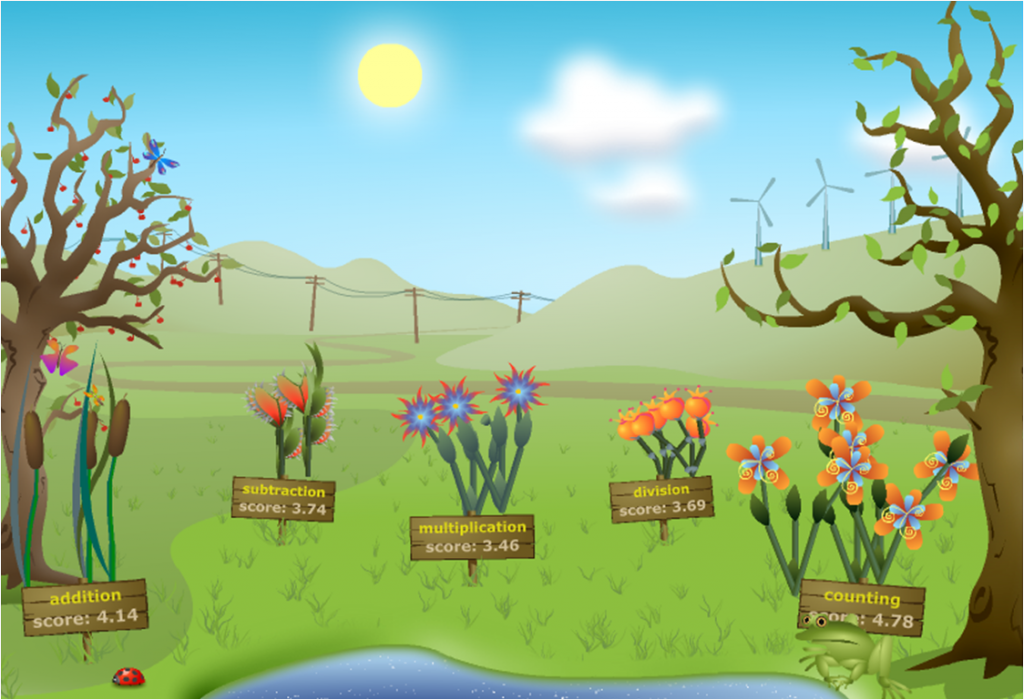
\includegraphics[width=0.4\textwidth]{images/mathsgarden.png} \label{fig_mathsgarden1}}
      \hfill
      \subfloat[решение задачи]{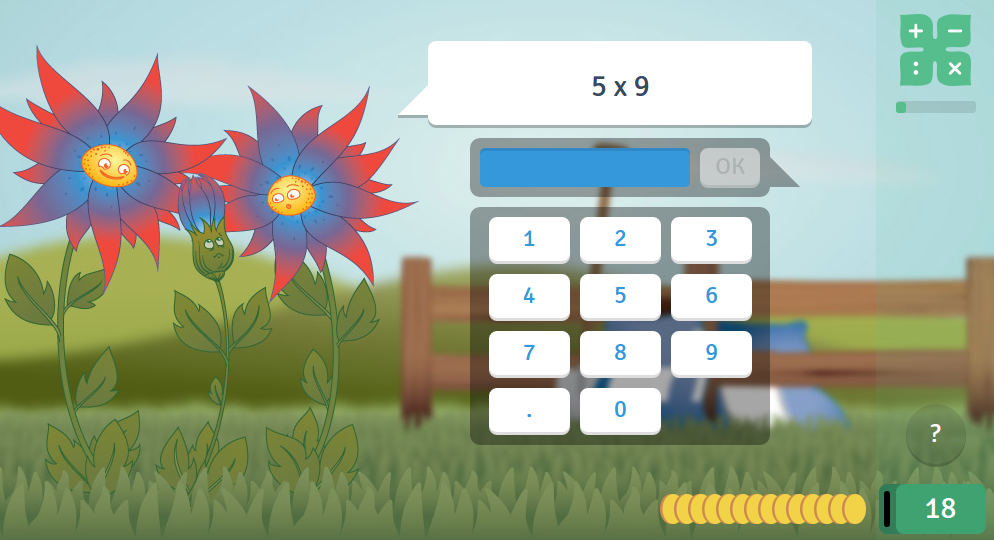
\includegraphics[width=0.5\textwidth]{images/mathsgarden_quiz.png} \label{fig_mathsgarden2}}
      
    \end{figure}
    
\end{frame}


\begin{frame}\frametitle{Адаптивные рекомендации: \\подсчет сложности}
       \begin{columns}
          \column{0.58\linewidth}
              Elo chess rating
              \begin{itemize}
                \item Арпад Эло, 1978\cite{elo1978rating}
                \item $E(S_j) = \frac{1}{1 + 10 ^ {(\theta_j - \theta_k) / 400}}$, \\где $\theta_j$ и $\theta_k$ -- рейтинги игроков, $S_j \in \{0, 0.5, 1\}$
                \item $\hat{\theta_j} = \theta_j + K(S_j - E(S_j))$
                \item Марк Гликман, 1995: пусть $K$ -- не const \cite{glickman95}
              \end{itemize}
           \column{0.38\linewidth}
              \centering
              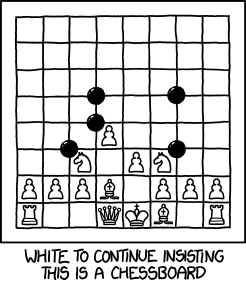
\includegraphics[height=5cm, width=3.5cm]{images/chess.png}
         \end{columns} 
\end{frame}



\begin{frame}\frametitle{Результаты: обычные рекомендации}
\bigskip

\begin{table}[H]
    \begin{tabular}{| c || r| }
      Метрика & Значение \\
      \hline		
      Число сессий & 381868 \\
      Число сессий с реакцией & 18066 \\
      Процент сессий с реакцией &  4.7\% \\
      Число открытых рекомендаций (из 20) & 1.6 \\
      Пройденная часть урока & 0.52 \\
      Число отказов от рекомендации & 184 \\\hline
    \end{tabular}
\end{table}


\begin{figure}[H]
  \centering
  \subfloat[открыто ссылок]{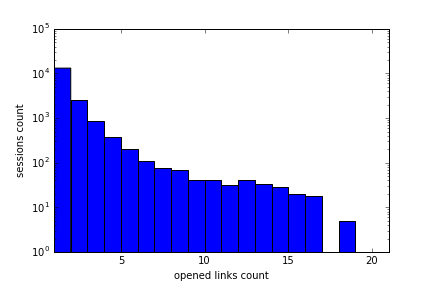
\includegraphics[width=0.4\textwidth]{images/home_page_opened_links_number_hist.png}}
  \hfill
  \subfloat[решено от задачи]{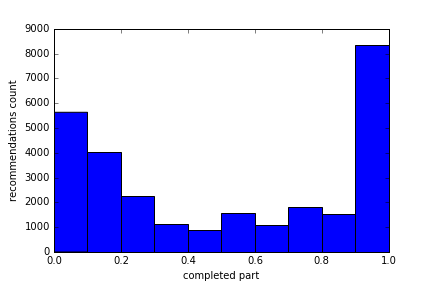
\includegraphics[width=0.4\textwidth]{images/home_page_completed_part_hist.png}}
\end{figure}

\end{frame}


\begin{frame}\frametitle{Результаты: контекстные рекомендации}

\bigskip

\begin{table}[H]
    \begin{tabular}{| c || r| }
      Метрика & Значение \\
      \hline		
      Число сессий & 26995 \\
      Число сессий с реакцией & 15125 \\
      Процент сессий с реакцией &  56\% \\
      Число открытых рекомендаций (из 5) & 1.48 \\
      Пройденная часть урока & 0.5 \\
      Число отказов от рекомендации & 0 \\
      \hline  
    \end{tabular}
\end{table}

\begin{figure}[H]
  \centering
  \subfloat[открыто ссылок]{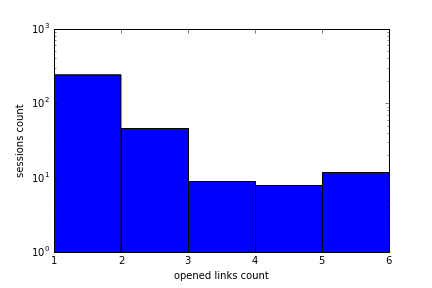
\includegraphics[width=0.4\textwidth]{images/context_opened_links_number_hist.png}}
  \hfill
  \subfloat[решено от задачи]{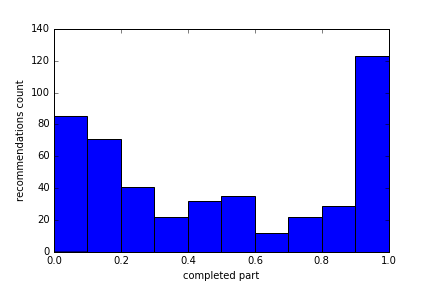
\includegraphics[width=0.4\textwidth]{images/context_completed_part_hist.png}}
\end{figure}

\end{frame}


\begin{frame}\frametitle{Результаты: адаптивные рекомендации}

\begin{table}[H]
    \begin{tabular}{| c || r| }
      Метрика & Значение \\
      \hline		
      Число сессий & 1511 \\
      Число пользователей & 246 \\
      Реакций "решено" & 1329 \\
      Реакций "слишком просто" & 95 \\ 
      Реакций "слишком сложно" & 87 \\
      MSE предсказания исхода & 0.22 \\
      
     \hline  
    \end{tabular}
\end{table}

% Также было исследовано, действительно ли ошибка предсказания для конкретного пользователя или задачи уменьшается со временем. Для этого ошибки были усреднены по пользователям (рисунок \ref{fig:adapt1}) и по задачам (рисунок \ref{fig:adapt2}). На получившихся графиках наблюдается явное, хоть и не равномерное, убывание ошибки.


\begin{figure}[H]
  \centering
  \subfloat[пересчет знаний пользователя]{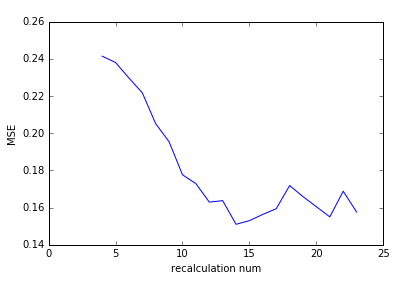
\includegraphics[width=0.45\textwidth]{images/mse_user_skill.png}}
  \hfill
  \subfloat[пересчет сложности задачи]{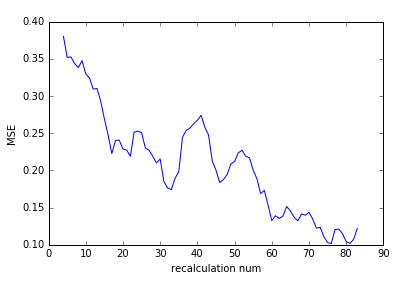
\includegraphics[width=0.45\textwidth]{images/mse_quiz_difficulty.png}}
\end{figure}

\end{frame}


\begin{frame}\frametitle{Планы}
    \begin{itemize}
        \item Развитие адаптивной системы:
            \begin{itemize}
                \item связи между материалами, темами
                \item дискриминативность и другие характеристики задач
            \end{itemize}
        \bigskip
        \item Более глубокий анализ накопленных данных
    \end{itemize}

\end{frame}


\begin{frame}\frametitle{Литература}
\setmonofont[Mapping=tex-text]{CMU Typewriter Text}
\bibliographystyle{ugost2008ls}
\bibliography{diploma.bib}
\end{frame}


\begin{frame}

\begin{columns}
  \column{0.38\linewidth}
      \huge{Спасибо! \\\indent \\\indent Вопросы?}
   \column{0.38\linewidth}
      \center{
\includegraphics[width=\linewidth]{images/stepic_all_clear.png}}
 \end{columns} 


\end{frame}


\end{document}